

\section{Membuat Data Vektor}
Disusun oleh:

Eko cahyono putro 1164035
Nur Arkhamia Batubara 1164049

\subsection {Pengertian Data Vektor}
Data vektor merupakan tipe data yang umum ditemukan dalam SIG. Sebuah vektor pada intinya merupakan sesuatu yang berbentuk sebuah titik, atau garis yang menghubungkan titik-titik tersebut. Dengan kata lain, titik, garis, dan poligon merupakan vektor (garis lengkung merupakan vektor juga).

Salah satu hal yang penting untuk dicatat adalah \textit{layer} QGIS hanya mengandung satu tipe fitur. Artinya, satu layer tidak dapat mengandung fitur titik dan fitur garis, karena mereka merupakan tipe data yang berbeda. Namun apabila anda ingin memiliki sebuah \textit{file} yang memiliki \textit{polygon} sekolah dan file lain yang memiliki titik-titik sekolah, anda dapat menambahkan mereka sebagai dua \textit{layer} yang terpisah\cite{setiawan2018membuka}.

\subsection{Tutorial Membuat data vektor}
Hal pertama yang harus dilakukan untuk membuat data vektor adalah :
\begin{enumerate}
\item Menginstall python 3.6.6

\begin{figure}[htbp]
\centering
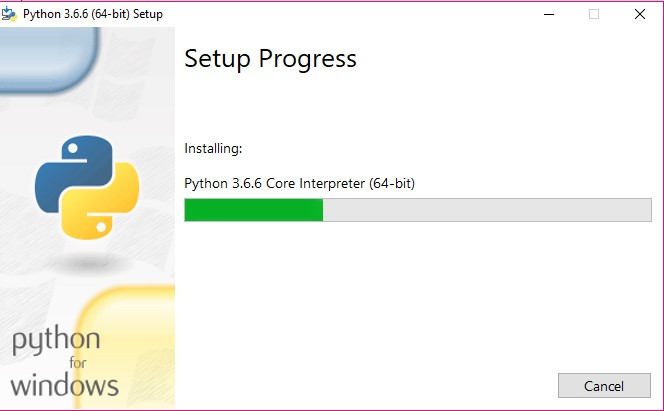
\includegraphics[width=0.75\textwidth]{pictures/python.jpg}
\caption{peroses instalasi \textit{python}}
\label{labelgambar1}
\end{figure}

\item Untuk mengecek apakan python sudah terinstall atau belum bisa menggunakan \textit{command prompt} pada computer anda.

\begin{figure}[htbp]
\centering
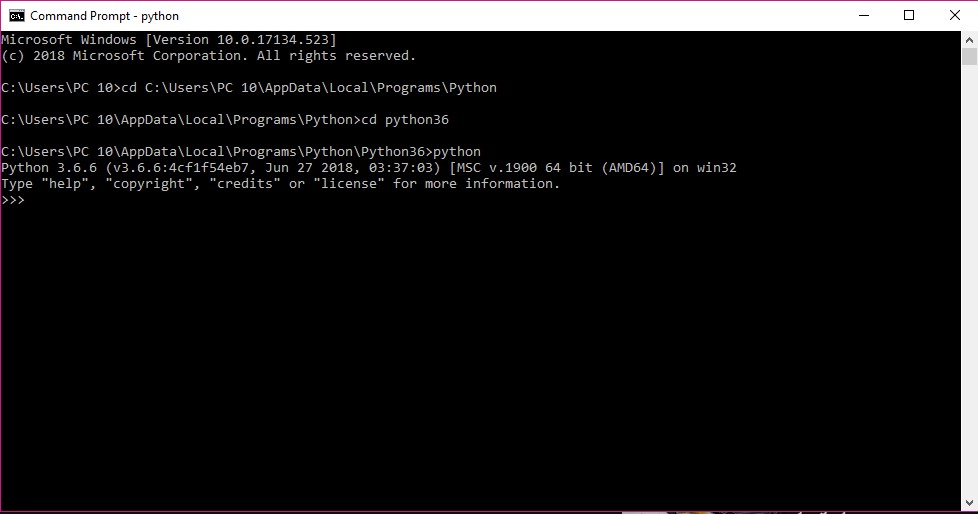
\includegraphics[width=0.75\textwidth]{pictures/pengecekanpython.jpg}
\caption{pengecekan \textit{python}}
\label{labelgambar2}
\end{figure}

Jika sudah muncul tampilan seperti digambar 1.2  ini maka python sudah terinstall.
\item Menginstall pyshp
\end{enumerate}

\begin{figure}[htbp]
\centering
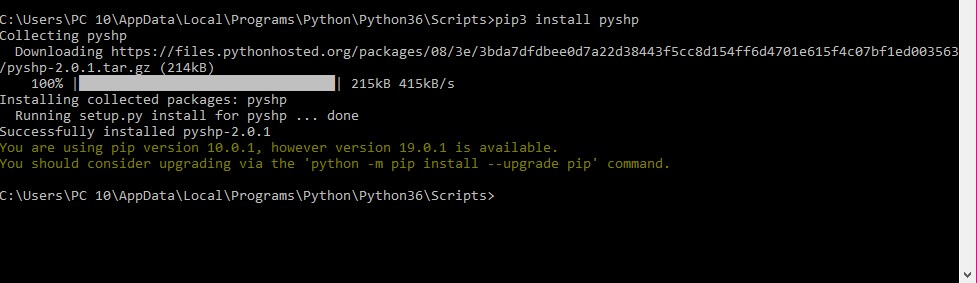
\includegraphics[width=1\textwidth]{pictures/installpy.jpg}
\caption{Mengintall Modul pyshp}
\label{labelgambar3}
\end{figure}
Kemudian menginstal modul pyshp dengan mengetik pip install pyshp di cmd. pyshp ini penting karena akan menggunakan modul ini untuk membuat data vector.Berikut langkah-langkah untuk membuat data vector yaitu beberapa bangun datar mulai dari point, polyline dan polygon. 

\subsection{Point}
Point adalah perintah untuk membuat sebuah titik. Adapun default-nya bentuk titik adalah noktah, akan tetapi bentuk tersebut bisa diubah sesuai dengan keinginan.

\begin{enumerate}
\item Untuk membuat file shp bisa menggunakan tools editor seperti notepad++, visualcode, sublime dan lain-lain, di sini saya menggunakan editor notepa+d+.  Buat script seperti gambar dibawah dan simpan dalam bentuk file .py:
\begin{figure}[htbp]
\centering
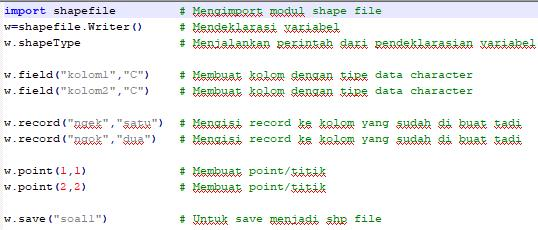
\includegraphics[width=1\textwidth]{pictures/soal1.jpg}
\caption{File Soal 1.py}
\label{labelgambar4}
\end{figure}

\item Jalankan program tersebut menggunakan \textit{command prompt}

\begin{figure}[htbp]
\centering
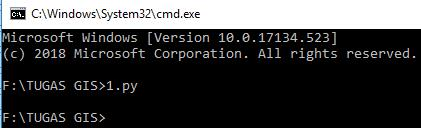
\includegraphics[width=1\textwidth]{pictures/pengujiansoal1.jpg}
\caption{Pengujian Soal1}
\label{labelgambar5}
\end{figure}
\end{enumerate}

\subsection{Tipe Data Geospasial}
Vektor dan data raster dua jenis data utama yang dipakai dalam Sistem Informasi Geospasial. Kedua vektor dan data raster mempunyai sistem referensi spasial. Ini adalah lintang dan bujur yang menentukan posisi di Bumi. Kita tahu ada dua model-model, yaitu data utama spasial vektor dan raster data. Tapi apa perbedaan antara raster dan vektor data? Kapan sebaiknya data ditampilkan sebagai raster atau vektor?
\begin{enumerate}
\item Vektor data tidak terdiri dari grid piksel. Sebaliknya, grafik vektor terdiri dari simpul dan jalur. Tiga jenis simbol dasar untuk data-data vektor adalah titik, garis dan poligon (untuk area). Sejak waktu subuh, peta tekah menggunakan simbol untuk mewakili fitur dunia nyata. Dalam terminologi Sistem Informasi Geospasial, fitur dunia nyata disebut dengan entitas spasial. 
Kegunaan Data Vektor Spatial Data Types adalah untuk menganalisa yang membutuhkan ketepatan posisi, misalnya pada basis data batas-batas kadaster: Contoh penggunaan lainnya adalah untuk mendefiniskan hubungan spasial dari beberapa fitur. Kelemahan data vektor yang utama adalah ketikmampuannya dalam mengakomodasi perubahan gradual. 

\end{enumerate}

